\section{Experiments}

\subsection{Experiment Environment}
We implemented our model using Python 3.6, Tensorflow 1.11 and Keras 2.2.
The model was trained on a single NVIDIA TITAN X (Pascal) GPU platform with ubuntu installed.


\subsection{Dataset}
We use the public dataset CelebA\upcite{celeba}, which contains 202,599 facial images, and 40 labelled attributes for each face.
We aligned and cropped the facial images into three-channel(RGB) images of 128×128 pixels and then divide them into training sets, test sets, and verification sets according to the ratio of 8:1:1.
For the 40 attributes in the dataset, we select 4 of them: 'gender', 'skin color', 'hair color', 'beard' attribute to verify the feasibility of the model.

\subsection{Experimental Items}
\begin{itemize}
\item In order to obtain a suitable model structure and training hyperparameters, we designed multiple sets of comparative experiments to test the effects of different improvement projects.
\item In order to verify that our model can generate facial images with high realism according to input conditions, and it has practicability, we set up the experiment of generating and adjusting facial images.
\item To prove that our method is cheaper to use, we also set up a set of model size comparison experiments.
\end{itemize}

\subsection{Training Details}

We use the Adam\upcite{adam} optimizer to optimize the network.
The learning rates of discriminator, generator and adjustor network are set to $1\times10^{-4}$.
$\beta1$ and $\beta2$ select the default configuration in Adam's\upcite{adam} paper, which is respectively 0.5 and 0.9.
Eecoder network is freezed when training adjustor network.
The $\lambda$ in both generator and adjustor network is set to 0.02.
We use 128-dimensional latent vector as input.
Use 32 images training set for training.
A total of 25 training sessions are used.
In each batch, generator is used to generate the image first.
Then discriminator is used to identify the image and adjusted by adjustor network.
The calculation results above are on gradient penalization and the respective losses of discriminator, generator, and adjustor network are calculated.
Then the respective optimizers separately performs backpropagation and optimizes network weight parameters.
In the partition training, the overall model training and the partition training are performed in a 4:1 ratio.

\subsection{Experiment Result}
\subsubsection*{More efficient image generation}
Figure \ref{littlegan_e1} and Figure \ref{dcgan_e1} show the results after training 1 epoch of training on LittleGAN and DCGAN\upcite{dcgan} on the CelebA\upcite{celeba} training set.
LittleGAN has been able to produce clear, highly recognizable facial images after training 1 epoch of training.
Compared to our DCGAN\upcite{dcgan}, we can clearly see that the images generated by LittleGAN are sharper and clearer.
It is also closer to the real image in color.

\begin{figure}
    \begin{minipage}[t]{0.48\linewidth}
        \centering
        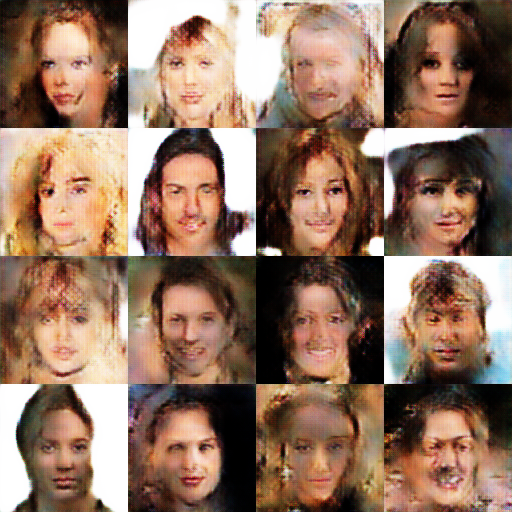
\includegraphics[width=\textwidth]{figures/result_littlegan_e1.png}
        \caption{Test result of LittleGAN after training 1 epoch}
        \label{littlegan_e1}
    \end{minipage}
        \hfill
    \begin{minipage}[t]{0.48\linewidth}
        \centering
        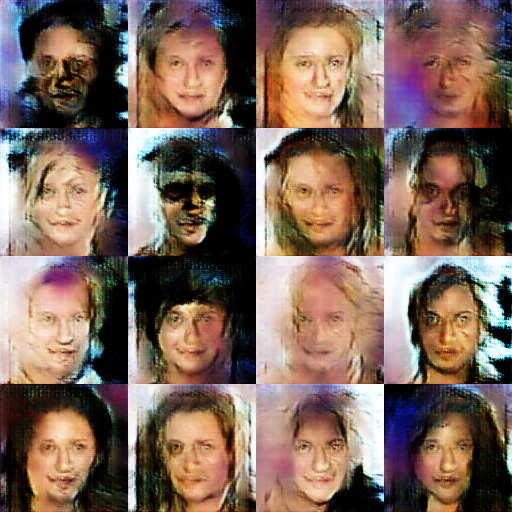
\includegraphics[width=\textwidth]{figures/result_dcgan_e1.png}
        \caption{Test result of DCGAN after training 1 epoch}
        \label{dcgan_e1}
    \end{minipage}
\end{figure}

\subsubsection*{More Stable}
Figure \ref{loss_part_on_d} and \ref{loss_dcgan_d} are the Discriminator's loss changes of LittleGAN and DCGAN\upcite{dcgan}.
Figure \ref{loss_part_on_g} and \ref{loss_dcgan_g} are the Generator's loss changes of LittleGAN and DCGAN\upcite{dcgan}.
To better measure the convergence speed of LittleGAN and DCGAN\upcite{dcgan}, we use the TensorBoard visualization tool to generate a loss map of the network during training.
By comparison, it can be found that compared with DCGAN\upcite{dcgan}, the loss of our network changes more smoothly, the jitter is smaller and is steadily decreasing.
While DCGAN\upcite{dcgan} often appears to have a fitting and lead to a sudden increase in loss.

\begin{figure}
    \begin{minipage}[t]{0.49\linewidth}
        \centering
        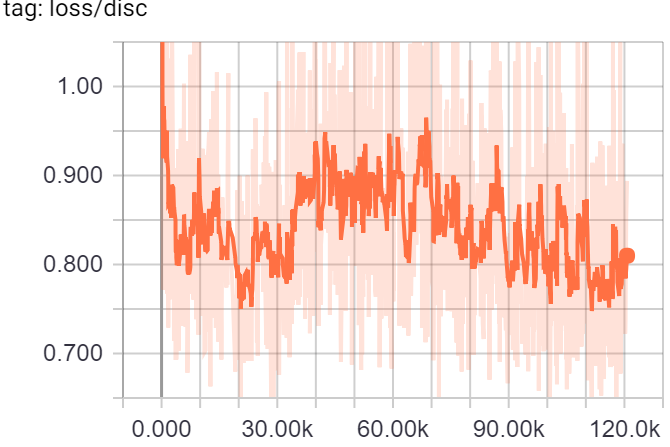
\includegraphics[width=\textwidth]{figures/loss_part_on_d.png}
        \caption{Loss line chart of LittleGAN's Discriminator (turn partition training on)}
        \label{loss_part_on_d}
    \end{minipage}
        \hfill
    \begin{minipage}[t]{0.49\linewidth}
        \centering
        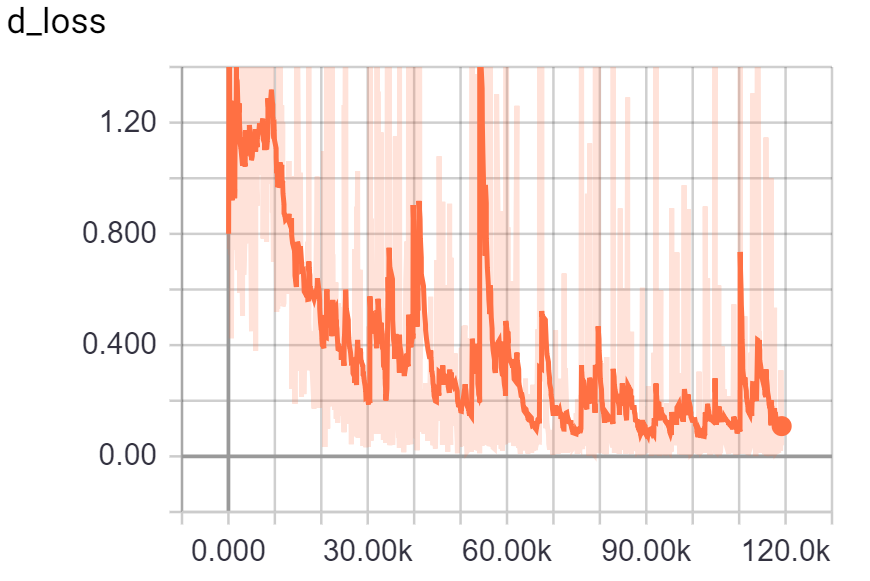
\includegraphics[width=\textwidth]{figures/loss_dcgan_d.png}
        \caption{Loss line chart of DCGAN's Discriminator}
        \label{loss_dcgan_d}
    \end{minipage}
\end{figure}

\begin{figure}
    \begin{minipage}[t]{0.49\linewidth}
        \centering
        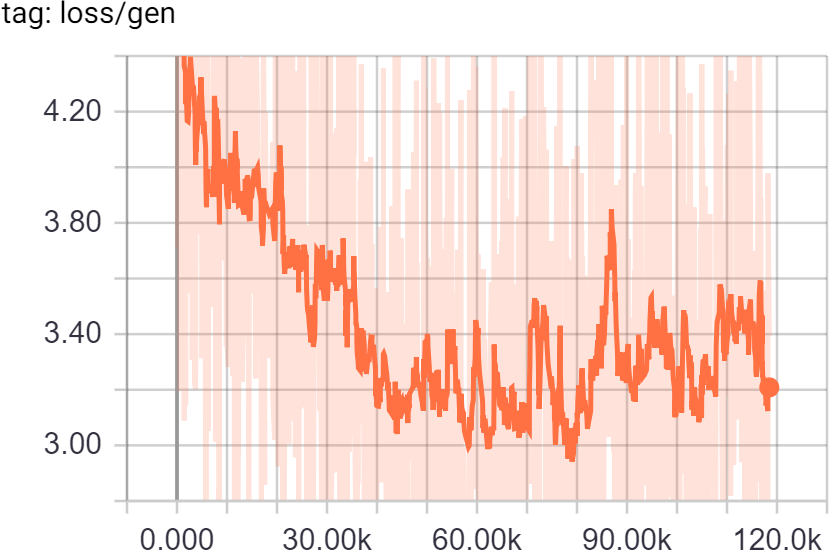
\includegraphics[width=\textwidth]{figures/loss_part_on_g.png}
        \caption{Loss line chart of LittleGAN's Generator (turn partition training on)}
        \label{loss_part_on_g}
    \end{minipage}
        \hfill
    \begin{minipage}[t]{0.49\linewidth}
        \centering
        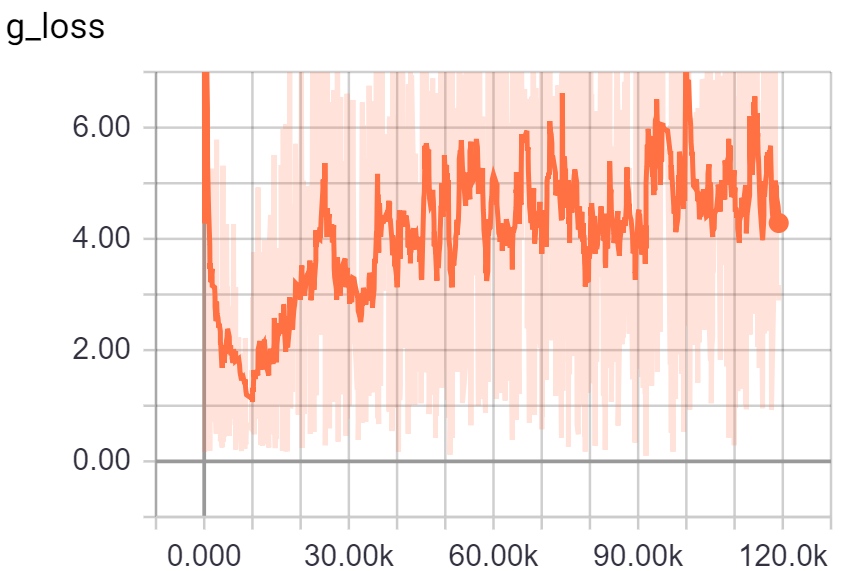
\includegraphics[width=\textwidth]{figures/loss_dcgan_g.png}
        \caption{Loss line chart of DCGAN's Generator}
        \label{loss_dcgan_g}
    \end{minipage}
\end{figure}

Figure \ref{littlegan_e15} and Figure \ref{dcgan_e15} are the test output of LittleGAN and DCGAN\upcite{dcgan} after training 15 epochs of training.
LittleGAN could output very authentic facial images after training 15 epochs.
In our experiment, mode collapse occurred on DCGAN\upcite{dcgan} after training 16 epochs, which led to the failure of network training.

\begin{figure}
    \begin{minipage}[t]{0.48\linewidth}
        \centering
        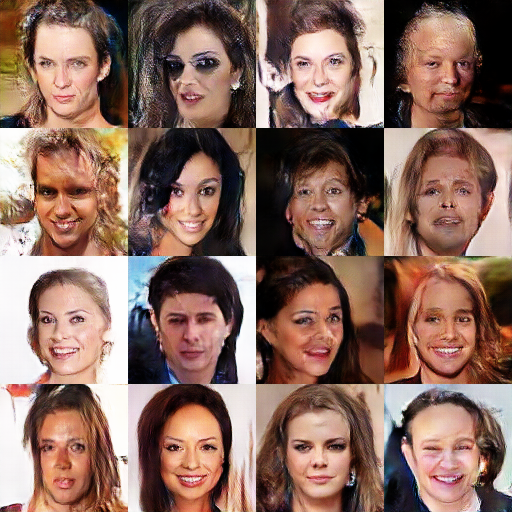
\includegraphics[width=\textwidth]{figures/result_littlegan_e15.png}
        \caption{Test result of LittleGAN after training 15 epochs}
        \label{littlegan_e15}
    \end{minipage}
        \hfill
    \begin{minipage}[t]{0.48\linewidth}
        \centering
        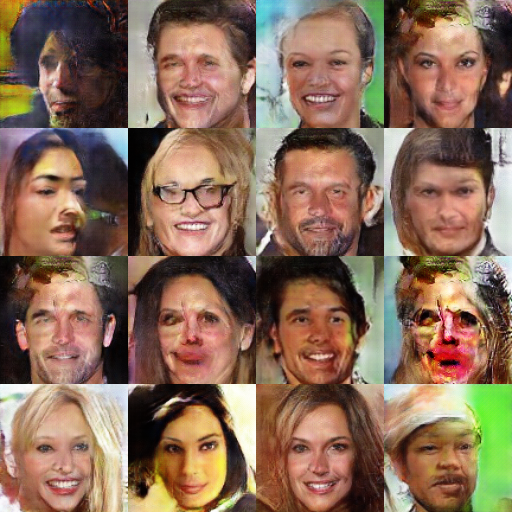
\includegraphics[width=\textwidth]{figures/result_dcgan_e15.png}
        \caption{Test result of DCGAN after training 15 epochs}
        \label{dcgan_e15}
    \end{minipage}
\end{figure}


\subsubsection*{Less Information Loss}
Figure \ref{adjust} is the test result of the generation and adjustment of the facial image.
It can be seen that when the image is roughly consistent, a single feature appears different from other images and other features are not lost.
Our network is able to adjust the specified features of the facial image.

\begin{figure}
    \begin{center}
    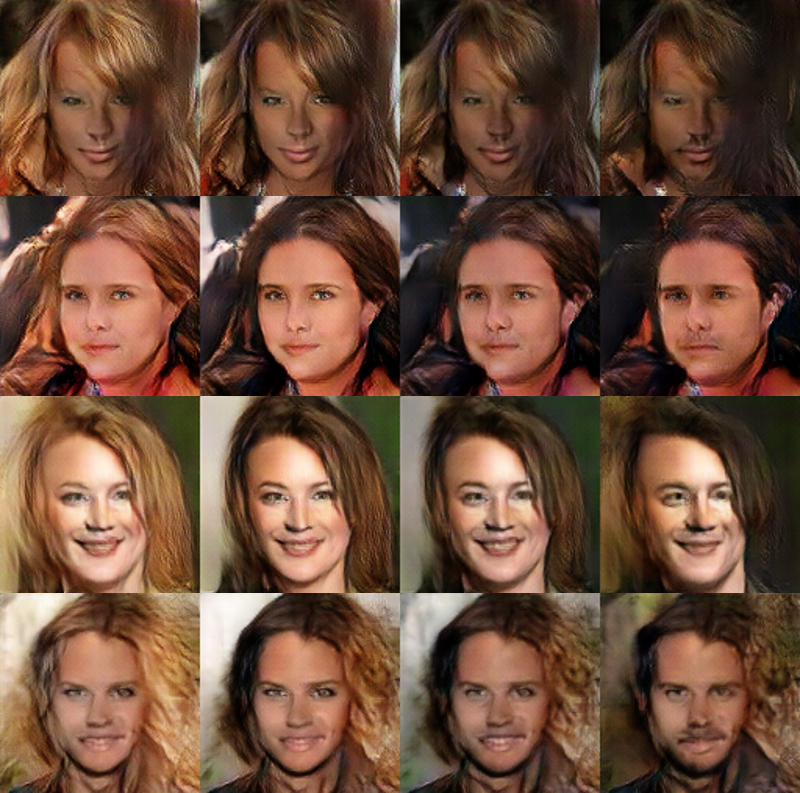
\includegraphics[width=0.49\textwidth]{figures/result_adjust_1.png}
    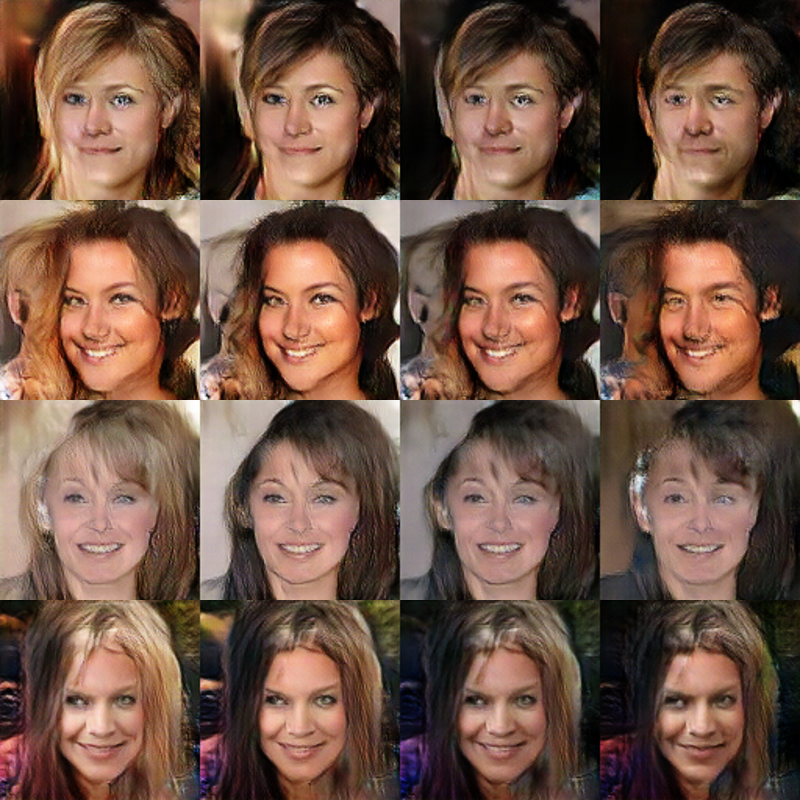
\includegraphics[width=0.49\textwidth]{figures/result_adjust_2.png}
    \caption{Adjustment test result of LittleGAN's Adjustor}
    \label{adjust}
    \end{center}
\end{figure}

\subsubsection*{Faster Convergence}
Fig.\ref{loss_part_on_d}, Fig.\ref{loss_part_on_g}, and Fig.\ref{loss_part_on_u} show the changes of the loss of each components that turn partition training off, respectively.
Fig.\ref{loss_part_off_d}, Fig.\ref{loss_part_off_g}, and Fig.\ref{loss_part_off_u} show the changes of the loss of each components that turn partition training off, respectively.
It can be seen that the loss of generator reaches the balance faster after partition training is started and the loss of discriminator also has a small amplitude and becomes stable.
Figure \ref{part_on} and Figure \ref{part_off} show the test output of the partition training on and off, respectively.
after training 20 epochs, with partition training on, image quality is improved under the same training amount.

\begin{figure}
    \begin{minipage}[t]{0.48\linewidth}
        \centering
        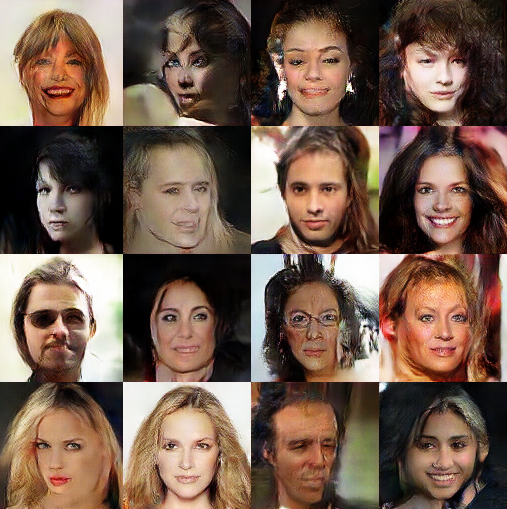
\includegraphics[width=\textwidth]{figures/result_part_on.png}
        \caption{Test result after training 20 epochs (turn partition training on)}
        \label{part_on}
    \end{minipage}
        \hfill
    \begin{minipage}[t]{0.48\linewidth}
        \centering
        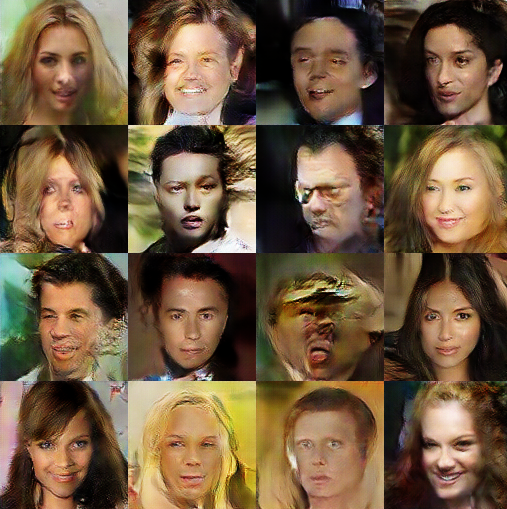
\includegraphics[width=\textwidth]{figures/result_part_off.png}
        \caption{Test result after training 20 epochs (turn partition training off)}
        \label{part_off}
    \end{minipage}
\end{figure}

\begin{figure}
    \begin{minipage}[t]{0.49\linewidth}
        \centering
        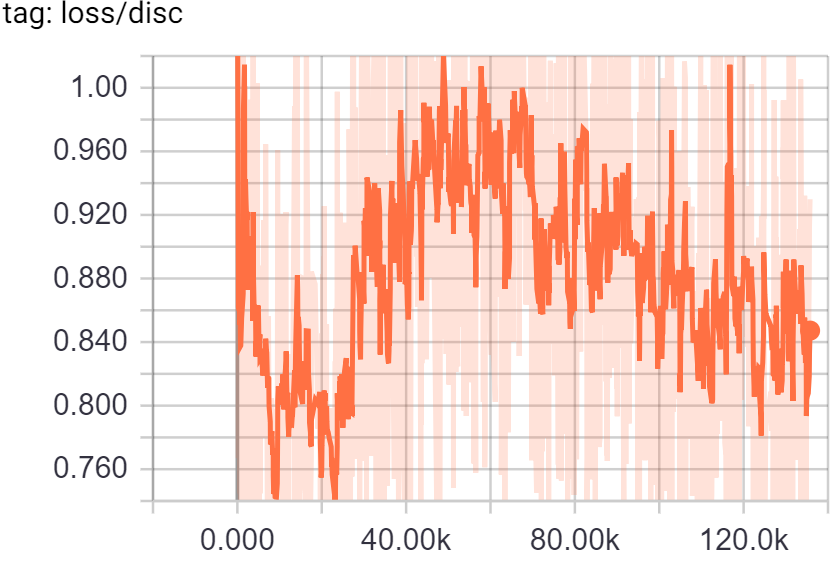
\includegraphics[width=\textwidth]{figures/loss_part_off_d.png}
        \caption{Loss line chart of LittleGAN's Discriminator (turn partition training off)}
        \label{loss_part_off_d}
    \end{minipage}
        \hfill
    \begin{minipage}[t]{0.49\linewidth}
        \centering
        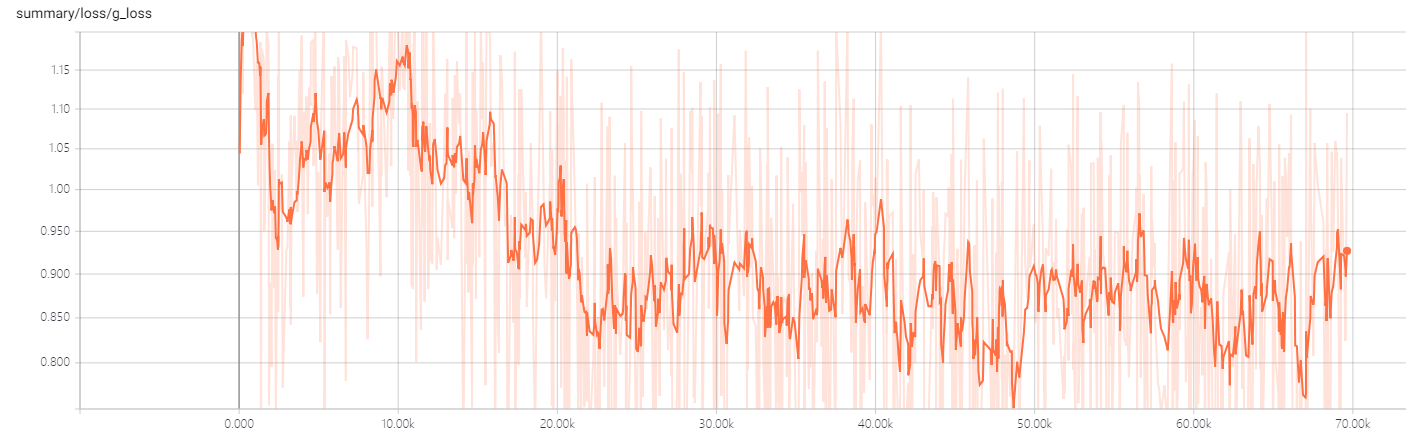
\includegraphics[width=\textwidth]{figures/loss_part_off_g.png}
        \caption{Loss line chart of LittleGAN's Generator (turn partition training off)}
        \label{loss_part_off_g}
    \end{minipage}
\end{figure}

\begin{figure}
    \begin{minipage}[t]{0.49\linewidth}
        \centering
        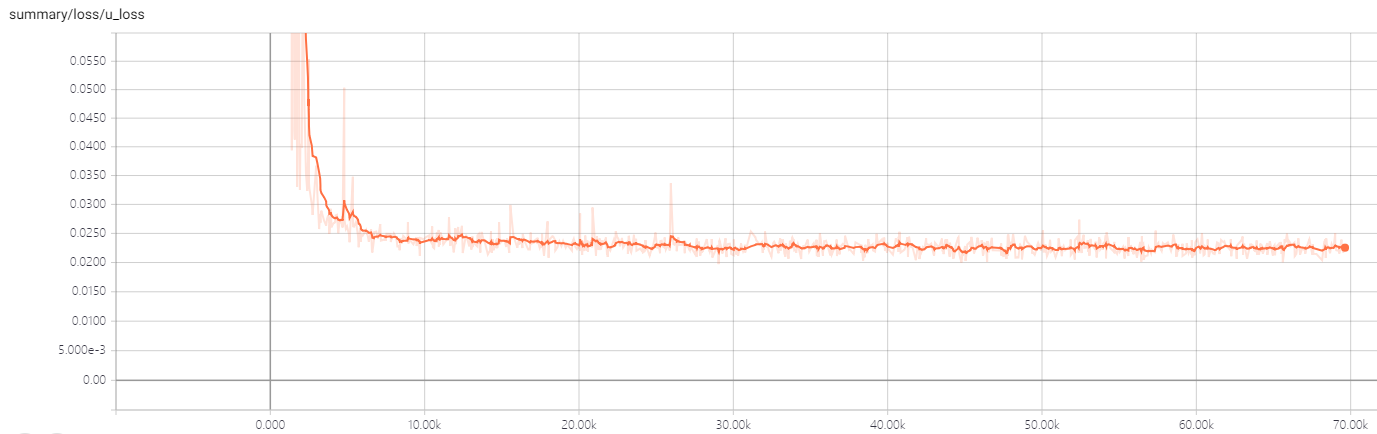
\includegraphics[width=\textwidth]{figures/loss_part_off_u.png}
        \caption{Loss line chart of LittleGAN's Adjustor (turn partition training off)}
        \label{loss_part_off_u}
    \end{minipage}
        \hfill
    \begin{minipage}[t]{0.49\linewidth}
        \centering
        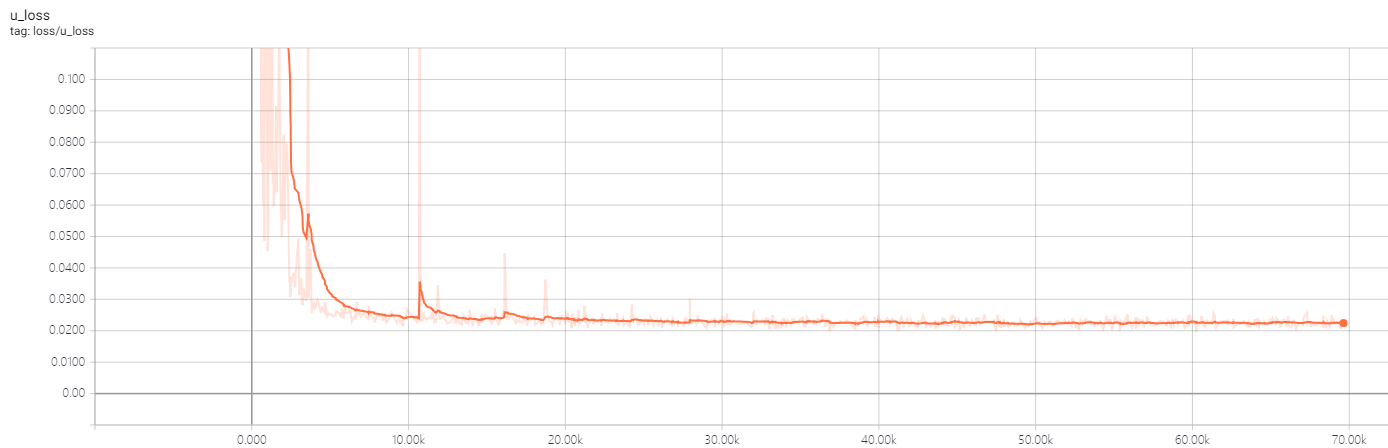
\includegraphics[width=\textwidth]{figures/loss_part_on_u.png}
        \caption{Loss line chart of LittleGAN's Adjustor (turn partition training on)}
        \label{loss_part_on_u}
    \end{minipage}
\end{figure}


\subsubsection*{Lower Use-cost}
We have used a variety of methods to reduce the size of model and the amount of computation.
We compared model size of pix2pix\upcite{pix2pix}, DCGAN\upcite{dcgan} and LittleGAN when outputting the same size image (a three-channel color image of 128 × 128 pixels).
(As shown in Figure \ref{result_model_size}).
It can be seen that the size of LittleGAN is smaller and LittleGAN costs less.

\begin{figure}
    \begin{center}
    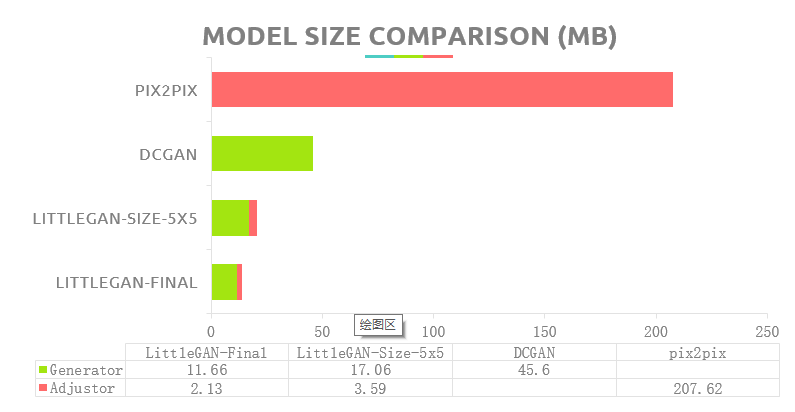
\includegraphics[width=\textwidth]{figures/result_model_size.png}
    \caption{Model Size Comparison}
    \label{result_model_size}
    \end{center}
\end{figure}